% ------ headers globales y begin ---------------
\documentclass[11pt, a4paper, twoside]{article}
\usepackage{header_tp1}
\begin{document}{}
% -----------------------------------------------

\subsubsection{Descripción}

Dada una cantidad $n$ de pizzas $i$ de orfebrería, cada una de las cuales tienen
una pérdida diaria de ganancia $d_i$ y una cantidad de días $t_i$ que lleva su
fabricación, se quiere saber el orden en que el pizzero Franco Shar tendría que
fabricar y vender las mismas para minimizar las pérdidas. Cada pizza no
entregada pasadas las media hora dará como mínimo una pérdida de $d_i$ por
$t_i$, y a esto se le sumará $d_i$ por la cantidad de días que Frank haya estado
fabricando otras pizzas, ya que él sólo puede trabajar de a una pizza a la vez.
El problema se deberá resolver con una complejidad temporal de
$\mathcal{O}(n^{2})$, siendo $n$ la cantidad de pizzas a fabricar. En el
resultado se mostrarán: $P$, el monto total perdido de la ganancia, y las pizzas
$i1,...,in$ ordenadas.


\begin{ejemplo}\hspace{1em}

	Frank tiene que entregar $n=3$ piezas en total ($i:1,2,3$). 

	Los datos de cada pieza $i$ son los siguientes:

	\begin{center}
		\begin{tabular}{|l|l|l|}
			\hline
			Pieza &  Pérdida diaria & $\#$ días de fabr.\\
			\hline
			$1$   &     $1$         & $3$               \\
			\hline 
			$2$   &     $2$         & $3$               \\
			\hline 
			$3$   &     $3$         & $3$               \\
			\hline 
		\end{tabular}
	\end{center}

	La fabricación de las $3$ piezas le llevará $9$ días en total y durante estos
	días se irán sumando las pérdidas diarias de ganancia correspondiente a cada
	pieza sin terminar.

	
		\begin{itemize}[leftmargin=+6em]
			\item[Día 1:] $3+2+1$. 
			\item[Día 2:] $3+2+1$. 
			\item[Día 3:] $3+2+1$ $\rightarrow$ entrega pizza $3$.
			\item[Día 4:] $2+1$.
			\item[Día 5:] $2+1$. 
			\item[Día 6:] $2+1$ $\rightarrow$ entrega pizza $2$.
			\item[Día 7:] $1$
			\item[Día 8:] $1$
			\item[Día 9:] $1$ $\rightarrow$ entrega pizza $1$.
		\end{itemize}

	
		

	Como resultado se obtendría el orden $3,2,1$ y $P:30$, el monto total perdido
	de la ganancia.
\end{ejemplo}

\begin{ejemplo}\hspace{1em}

	Frank tiene que entregar $n=2$ piezas en total ($i:1,2$). Los datos de cada pieza $i$ son los siguientes: \\

	\begin{center}
		\begin{tabular}{|l|l|l|}
			\hline
			Pieza &  Pérdida diaria & $\#$ días de fabr.\\
			\hline
			$1$   &     $1$         & $3$               \\
			\hline 
			$2$   &     $3$         & $1$               \\
			\hline 
		\end{tabular}
	\end{center}
	    
	La fabricación de las $2$ piezas le llevará $4$ días en total y durante estos días se irán sumando las pérdidas 
	diarias de ganancia correspondiente a cada pieza sin terminar. 

	\begin{itemize}[leftmargin=+6em]
		\item Día1: $3+1$ $\rightarrow$ entrega pieza $2$. 
		\item Día2: $1$. 
		\item Día3: $1$.
		\item Día4: $1$ $\rightarrow$ entrega pieza $1$.
	\end{itemize}  	
		
	Como resultado se obtendría el orden $2,1$ y $P:7$, el monto total perdido de la ganancia. 


\end{ejemplo}

\subsubsection{Hipótesis de resolución}

Tenemos $n$ pizzas, cada una de los cuales cuenta con un valor de $d$, es lo que
se va devaluando diariamente, y $t$, el tiempo que tomará su fabricación. Nos
interesa minimizar la pérdida de la ganancia total, dando el mejor orden en que
habría que ir fabricando las piezas $(1,...,n)$.

Definimos un cociente $\pi$ como $d/t$ para cada uno de los $n$ elementos. La
relación entre $d$ y $t$ es la que nos determinará cuál es el orden óptimo de
fabricación.

Contamos con un vector $v = (v_1,v_2,...,v_n)$. Cada $v_i$ representa la pieza
$i$ a fabricar, $i=1,...,n$.

Nuestro algoritmo ordena de forma decreciente por el cociente $\pi$, luego
devolvemos un vector $v$ óptimo.

Iteramos sobre $v$ con el indice $i$, acumulando la pérdida del subvector
v[1..i]. Al final de las iteraciones tenemos entonces la pérdida completa
correspondiente al vector $v$.


\subsubsection{Justificación formal de correctitud}

Contamos con $n \in \mathbb{N}$, donde cada collar queda determinado por una \texttt{3-upla}: ($p$,$d$,$t$) donde \\
$p \in \{1,...,n\}$ es el número de collar $(p_i \neq p_j)$, \\
$d \in \mathbb{N}$ es la pérdida diaria de ganancia del collar, y \\
$t \in \mathbb{N}$ es el tiempo de fabricación (en días) del collar. \\
Se pide devolver el orden de fabricación de los collares que minimice la pérdida total. \\
El espacio de soluciones es luego, todos los vectores que son permutaciones de los primeros $n$ naturales. \\
\\
Sea $v = (v_1,v_2,...,v_n)$ y entiéndase, \\
$d[V_i]$ como la segunda componente del collar que tiene $p=v_i$ \\
$t[V_i]$ como la tercer componente del collar que tiene $p=v_i$. \\
Sea $\displaystyle{C(V)= \sum_{i=1}^{n} ((\sum_{j=1}^{i} t[v_i])d[v_i])}$ la función que queremos minimizar sobre el espacio de soluciones. La \underline{solución} $v$ cumple $(\forall V')$ C(v) $\le$ C(v').\\
Para cada $i \in 1,...n$ consideramos $\displaystyle{ \pi(i)= \frac{d[v_i]}{t[v_i]}}$. \\
Veamos que $v$ cumple $\displaystyle{(\forall i \in 1...n-1) \pi(i) \ge \pi(i+1)}$. \\
\\
Supongo que no, es decir, $\displaystyle{(\exists X \in 1...n-1) \pi(X) < \pi(X+1)}$. \\
\\
Sea V'$=(v_1,v_2,...,v_{X-1},v_{X+1},v_X,v_{X+2},...,v_n)$, es decir, se construye a partir de V con las posiciones X e X$+1$ intercambiadas. \\
Veamos que C(v')$<$C(v). \\
\\
C(v)$-$C(v')$= \displaystyle {\sum_{i=1}^{n} (d[v_i](\sum_{j=1}^{i} t[v_j]))- \sum_{i=1}^{n}(d[v'_i](\sum_{j=1}^{i} t[v'_j]))} = $\\

$ \underbrace{\sum_{i=1}^{x-1} (d[v_i]\sum_{j=1}^{i} t[v_j]-\sum_{i=1}^{x-1}d[v'_i]\sum_{j=1}^{i} t[v'_j]}_{0,\textnormal{ pues} \forall i \in 1...x-1, v_i=v'_i}$ + 
$\displaystyle{d[v_x]\sum_{j=1}^{x} t[v_j] - d[v'_x]\sum_{j=1}^{x}t[v'_j] +}$ \\ 
$\displaystyle{d[v_{x+1}]\sum_{j=1}^{x+1} t[v_j] - d[v'_{x+1}]\sum_{j=1}^{x+1}t[v'_j] + }$ 
$\underbrace{\sum_{i=x+2}^{n} (d[v_i]\sum_{j=1}^{i} t[v_j]-\sum_{i=x+2}^{n}d[v'_i]\sum_{j=1}^{i} t[v'_j]}_{0,\textnormal{ pues} \forall i \in x+2...n, v_i=v'_i \textnormal{y} \sum_{j=1}^{i}t[v_j]=\sum_{j=1}^{i}t[v'_j]} =$ \\
$\displaystyle{d[v_x](\sum_{j=1}^{x-1} t[v_j]+ t[v_x]) - d[v_{x+1}](\sum_{j=1}^{x-1} t[v_j] + t[v_{x+1}]) + }$ \\
$\displaystyle{d[v_{x+1}](\sum_{j=1}^{x-1} t[v_j] + t[v_x] + t[v_{x+1}]) - d[v_x](\sum_{j=1}^{x-1} t[v_j] + t[v_{x+1}] + t[v_x])=} $\\
$\displaystyle{-d[v_x] t[v_{x+1}] + d[v_{x+1}] t[v_x] > 0 \Leftrightarrow \frac{d[v_{x+1}]}{t[v_{x+1}]} > \frac{d[v_x]}{t[v_x]} } \Leftrightarrow $ \\
$\displaystyle{\pi(x+1) > \pi(x) }$ que asumimos como verdadero. \\
Abs! Pues $v$ era óptimo. Luego, $(\forall i \in 1...n-1) \pi(i) \ge \pi(i+1)$. \\
\\
Sabemos pues $v$ óptimo $\Rightarrow v$ ordenado no ascendentemente por $\pi$. \\
Sabemos que existe $v*$ óptima, luego existte $v*$ óptima y ordenada. \\
Veamos que $v$ ordenada $\Rightarrow v$ óptima, es decir que no existe $v$ ordenada y no óptima. \\
\\
C(v)$=$C(v*) pues uno siempre puede ir intercambiando dos posiciones $x$ y $x+1$ que mantengan el ordenamiento (es decir $\pi(x)=\pi(x+1))$ las veces que sea necesario hasta que $v=v*$ y luego, C(v)$=$C(v*) y por lo tanto, $v$ óptima. \\
\\
Veamos que se pueden intercambiar $x$ y $x+1$: \\
$v = (v_1,...,v_x,v_{x+1},...,v_n)$ \\
$v'= (v_1,...,v_{x+1},v_x,...,v_n)$ \\
\\
Desarrollando como hecho previamente, \\
$\displaystyle{C(v) - C(v') = -d[v_x]t[v_{x+1}] + d[v_{x+1}]t[v_x]=0 \Leftrightarrow }$\\
$\displaystyle{\frac{d[v_{x+1}]}{t[v_{x+1}]} = \frac{d[v_x]}{t[v_x]} \Leftrightarrow \pi(x+1) = \pi(x)}$ que asumimos verdadero. \\
\\
Luego, $v$ ordenado $\Rightarrow v$ óptimo. \\ 


\subsubsection{Cota de complejidad temporal}

\begin{algorithm}
\caption{La joya del Río de la plata}\label{alg:joyarioplata}
\footnotesize\begin{algorithmic}[1]
	\Require
		\Statex $cantidadDePiezas \gets$ \Call{dameCantidadDePiezas}{} \Comment{$integer$}
		\Statex $listaDePiezas \gets$ \Call{dameListaDePiezas}{} \Comment{$vector<Pieza>$}
	\Ensure
		\Statex \Call{Orden Óptimo Piezas}{} \Comment{$vector<Pieza>$}
	\Statex
	
  \State $sumaTotal \gets 0$ \Comment{\bigO{1}}
  \State $tiempoAcum \gets 0$ \Comment{\bigO{1}}
  \State \Call{ordenar}{listaDePiezas, \textsc{compararPiezasMayorQue} } \Comment{\bigO{n.\log n}}
  \ForAll {$pieza$ \texttt{en} $listaDePiezas$} \Comment {\texttt{n} iteraciones}
    \State $tiempoAcum \gets tiempoAcum + pieza.tiempo$ \Comment{ \bigO{1}}
    \State $sumaTotal \gets sumaTotal + pieza.devaluaci\acute{o}n * tiempoAcum $ \Comment{ \bigO{1}}
    \EndFor \Comment{\texttt{ciclo}\bigO{n}}
  \State \Return $listaDePiezas, sumaTotal$
  \State

  \Statex{}
  \Function{compararPiezasMayorQue}{$pieza1, pieza2$} \Comment{\bigO{1}}
  \If {$(pieza1.devaluaci\acute{o}n/pieza1.tiempo) > (pieza2.devaluaci\acute{o}n/pieza2.tiempo$} \Comment{\bigO{1}}
    \State \Return {1} \Comment{\bigO{1}}
  \Else
    \State \Return {0 \Comment{\bigO{1}}}
  \EndIf
	\EndFunction \Comment{\texttt{final} \bigO{1}}
  \State

  \Statex
  \State Definición \textbf{Pieza}:
  \State \texttt{ integer } tiempo \Comment{tiempo de fabricación}
  \State \texttt{ integer } devaluación \Comment{cantidad de dinero perdido por unidad de tiempo}
	\Statex{}
	
\end{algorithmic}
\end{algorithm}



  Como se puede ver en el pseudo código la complejidad está dada por un Ordenamiento.
El ordenamiento se realiza utilizando un criterio específico de comparación que consiste
en comparar el cociente entre la devaluación diaria de una pieza y el tiempo que toma
fabricar esa pieza. La comparación entonces tiene una complejidad de \bigO{1}, por lo que
un ordenamiento basado en comparaciones tiene complejidad de \bigO{n.\log n}.

  Luego hay un ciclo \textbf{para cada} que itera una por cada elemento en \textit{listaDePiezas},
por lo tanto el ciclo se realiza \textit{cantidadDePiezas} veces. Cada iteración del ciclo realiza
sólo acciones \bigO{1}, por lo tanto el ciclo en si es \bigO{cantidadDePiezas}. La cantidad de piezas
es proporcional al tamaño de la entrada, por lo tanto el ciclo es \bigO{n}.

  En conclusión el algorítmo tiene una complejidad temporal \bigO{n + n. \log n}=\bigO{n. \log n}

  




\subsubsection{Verificación mediante casos de prueba}

A continuación presentamos distintas instancias que sirven para verificar que el programa funciona correctamente: \\ 

\begin{minipage}{0.2\textwidth}
	\begin{tabular}{ll}
		Input  \\
		\hline
		n &  \\
		$d_1$ & $t_1$ \\
		\vdots & \vdots \\
		$d_n$ & $t_n$ 
	\end{tabular} \\ 
\end{minipage}
\begin{minipage}{0.2\textwidth}
	\begin{tabular}{ll}
		Output  \\
		\hline
		$i_1$ \dots $i_n$ & P \\
		 \\
		 \\
		 \\
	\end{tabular} \\ 
\end{minipage}  \\
\\
n: cant. total de piezas  \\
$d_i$: cant. de pérdida diaria de la pieza $i$ \\
$t_i$: cant. de días de fabricación ($1 \le i \le n$) \\
$i_1$ \dots $i_n$: n piezas ordenadas \\
P: monto total perdido de la ganancia \\

Podemos separar el conjunto de soluciones en los siguientes casos: 
\begin{enumerate}
    \item $\frac{d_i}{t_i}$ es igual  $\forall$ $i$. 
	
		\begin{minipage}{0.2\textwidth}
			\begin{tabular}{l}
				Input  \\
				\hline
				$3$   \\
				$2$ $1$ \\
				$4$ $2$ \\
				$8$ $4$ 
			\end{tabular} \\ 
		\end{minipage}
		\begin{minipage}{0.2\textwidth}
			\begin{tabular}{ll}
				Output  \\
				\hline
				$1$   $2$  $3$ & $70$ \\
				$1$   $3$  $2$ & $70$ \\
				\vdots         & \vdots\\
				$3$   $2$  $1$ & $70$ \\
			\end{tabular} \\ 
		\end{minipage}  \\
		\textnormal{Cualquier permutación de las piezas $1,2,3$ es una solución válida para este caso. $P=70$ en los $6$ posibles outputs. Esto es porque el cociente entre la pérdida diaria y el tiempo de fabricación es igual para las $3$ piezas, $\frac{d_i}{t_i}=2, \forall i = 1,2,3$.} \\

	\item $\exists$ $j$ tal que $\frac{d_i}{t_i}$ $\ne$ $\frac{d_j}{t_j}$, j $\ne$ i, con j, i $=$ $1,...,n$. 
	
	\begin{itemize}
		\item Fijo $t_i$ y varío $d_i$, $\forall$ $i$. Entonces el orden va a estar determinado por la pérdida diaria $d_i$.
		
		\begin{minipage}{0.2\textwidth}
			\begin{tabular}{l}
				Input  \\
				\hline
				$5$   \\
				$1$ $2$ \\
				$2$ $2$ \\
				$3$ $2$ \\
				$5$ $2$ \\
				$4$ $2$ \\
			\end{tabular} \\ 
		\end{minipage}
		\begin{minipage}{0.3\textwidth}
			\begin{tabular}{ll}
				Output  \\
				\hline
				$4$ $5$ $3$ $2$ $1$ & $70$ \\
				\\
				\\
				\\
			    \\
				\\
			\end{tabular} \\ 
		\end{minipage}  
		\begin{minipage}{0.2\textwidth}
			\begin{tabular}{l|l}
				Pieza i & $d_i$  \\
				\hline
				$1$ & $1$  \\
				$2$ & $2$ \\
				$3$ & $3$ \\
				$4$ & $5$ \\
				$5$ & $4$ \\
                        \\
			\end{tabular} \\ 
		\end{minipage}
		
		\item Fijo $d_i$ y varío $t_i$ $\forall$ $i$. El orden depende del cociente entre $d_i$ y $t_i$.
		
		\begin{minipage}{0.2\textwidth}
			\begin{tabular}{l}
				Input  \\
				\hline
				$3$   \\
				$2$ $1$ \\
				$2$ $2$ \\
				$2$ $3$ \\
			\end{tabular} \\ 
		\end{minipage}
		\begin{minipage}{0.3\textwidth}
			\begin{tabular}{ll}
				Output  \\
				\hline
				$1$ $2$ $3$ & $20$ \\
				\\
				\\
				\\
			\end{tabular} \\ 
		\end{minipage}  
		\begin{minipage}{0.2\textwidth}
			\begin{tabular}{l|l}
				Pieza i & $\frac{d_i}{t_i}$  \\
				\hline
				$1$     & $2$ \\
				$2$     & $1$ \\
				$3$     & $0,67$ \\
				\\
			\end{tabular} \\ 
		\end{minipage}  \\
		
		\item Varío $d_i$ y $t_i$ $\forall$ $i$ pero sin que todos los $\frac{d_i}{t_i}$ sean iguales. El orden depende del cociente entre $d_i$ y $t_i$. 
		
		\begin{minipage}{0.2\textwidth}
			\begin{tabular}{l}
				Input  \\
				\hline
				$3$   \\
				$3$ $1$ \\
				$1$ $2$ \\
				$2$ $3$ \\
			\end{tabular} \\ 
		\end{minipage}
		\begin{minipage}{0.3\textwidth}
			\begin{tabular}{ll}
				Output  \\
				\hline
				$1$ $3$ $2$ & $14$ \\
				\\
				\\
				\\
			\end{tabular} \\ 
		\end{minipage}  
        	\begin{minipage}{0.2\textwidth}
			\begin{tabular}{l|l}
				Pieza i & $\frac{d_i}{t_i}$  \\
				\hline
				$1$     & $3$ \\
				$2$     & $0,5$ \\
				$3$     & $0,67$ \\
				\\
			\end{tabular} \\ 
		\end{minipage}  \\		
		
	\end{itemize}
	
\end{enumerate}

Estos casos cubrirían todo el espacio de soluciones. Ejecutamos distintos ejemplos correspondientes a cada
uno de ellos y obtuvimos la respuesta esperada. Por lo tanto, podemos concluir que el comportamiento del programa 
es correcto. 

\newpage
\subsubsection{Medición empírica de la performance}

El algoritmo consta de dos partes, una de ordenamiento al principio, con complejidad \bigO{  cantPiezas . \log cantPiezas }
y una segunda parte que es sencillamente un recorrido por todas las piezas donde para cada pieza se hace
una multiplicación y una suma, por lo que claramente es lineal con respecto al tamaño de la entrada, pero no solo
en el peor caso sino que en cualquier caso. De esta manera el algorítmo pertenece a los de complejidad \bigO{n . \log n}.

Para contrastar esta idea de manera empírica lo que se hizo fue analizar el resultado del siguiente cociente: 

\begin{center}
$\frac{tiempoDeEjecuci\acute{o}n}{n. \log n}$
\end{center}

La figura \ref{fig:ej2-1} muestra el resultado de de este cociente para diferentes tamaños de la entrada.
Se puede apreciar que para tamaños de entrada grandes la curva se estabiliza muy cerca de una constante.
Este resultado reafirma la hipótesis de que el algorítmo pertenece a los de complejidad \bigO{n. \log n}


%Como la complejidad mayor está dada por la
%primer parte, decidimos enfocarnos en los parámetros de entrada que son tenidos en cuenta para dicho ordenamiento. 
%Estos son $d_i$ pérdida de ganancia diaria y $t_i$ tiempo de fabricación de la pieza. Lo que se termina ordenando 
%es el cociente $\pi=d_i/t_i$ de cada pieza $i$.\\
%Entonces, en la medición empírica de la performance del programa, realizamos pruebas comparando los tiempos según el
%ordenamiento dado de estos cocientes. Los casos son: 

%\begin{itemize}
%\item Orden ascendente de $\pi$. 
%\item Orden descendente de $\pi$ 
%\item Orden aleatorio de $\pi$. Se tomaron valores random de $d_i$ y $t_i$ para cada pieza $i$. 
%\end{itemize}     

%Para cada uno de los $3$ casos mencionados, tomamos los tiempos de ejecución variando la cantidad de piezas totales.\\
%Se puede observar en el gráfico $tiempo$ vs $n$ que la cota teórica calculada \bigO{n. \log n} fue correcta.  
 
%Gráfico

\begin{figure}[H]
   \begin{center}
   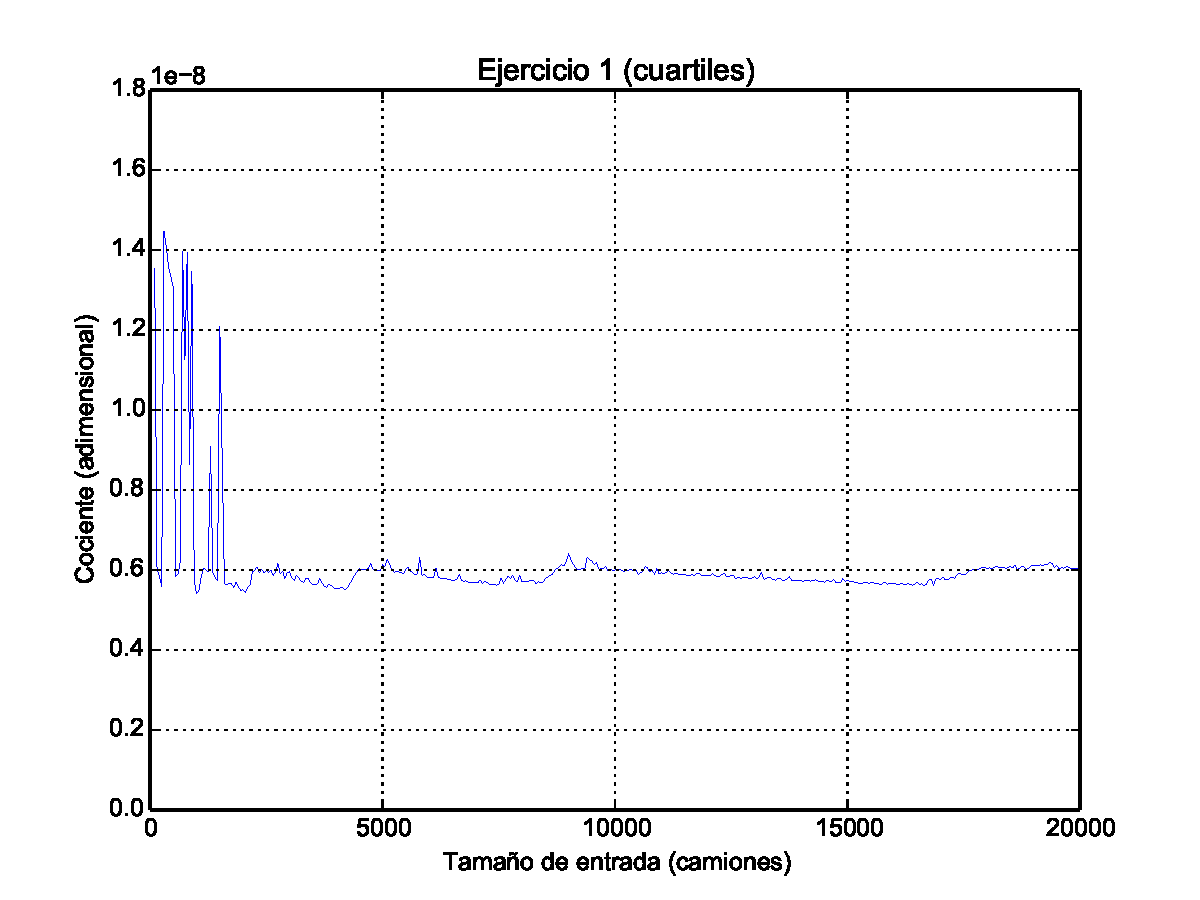
\includegraphics[width=1\textwidth,angle=0]{../ej2/graficos/test_2.pdf}
   \caption{}
   \label{fig:ej2-1}
   \end{center}
\end{figure}

% -----------------------------------------------
\end{document}
